\documentclass[11pt,a4paper]{scrartcl}
\usepackage[utf8x]{inputenc}
\usepackage{ucs}
\usepackage[english]{babel}
\usepackage{amsmath}
\usepackage{amsfonts}
\usepackage{amssymb}
\usepackage{dsfont}
\usepackage{graphicx}



\usepackage{pgf}
\usepackage{tikz}

\usetikzlibrary{arrows,automata}
\usetikzlibrary{positioning}

\usepackage[left=2cm,right=2cm,top=2cm,bottom=2cm]{geometry}
\author{Philipp Fröhlich}
\title{Classdiagram Overview}
\begin{document}


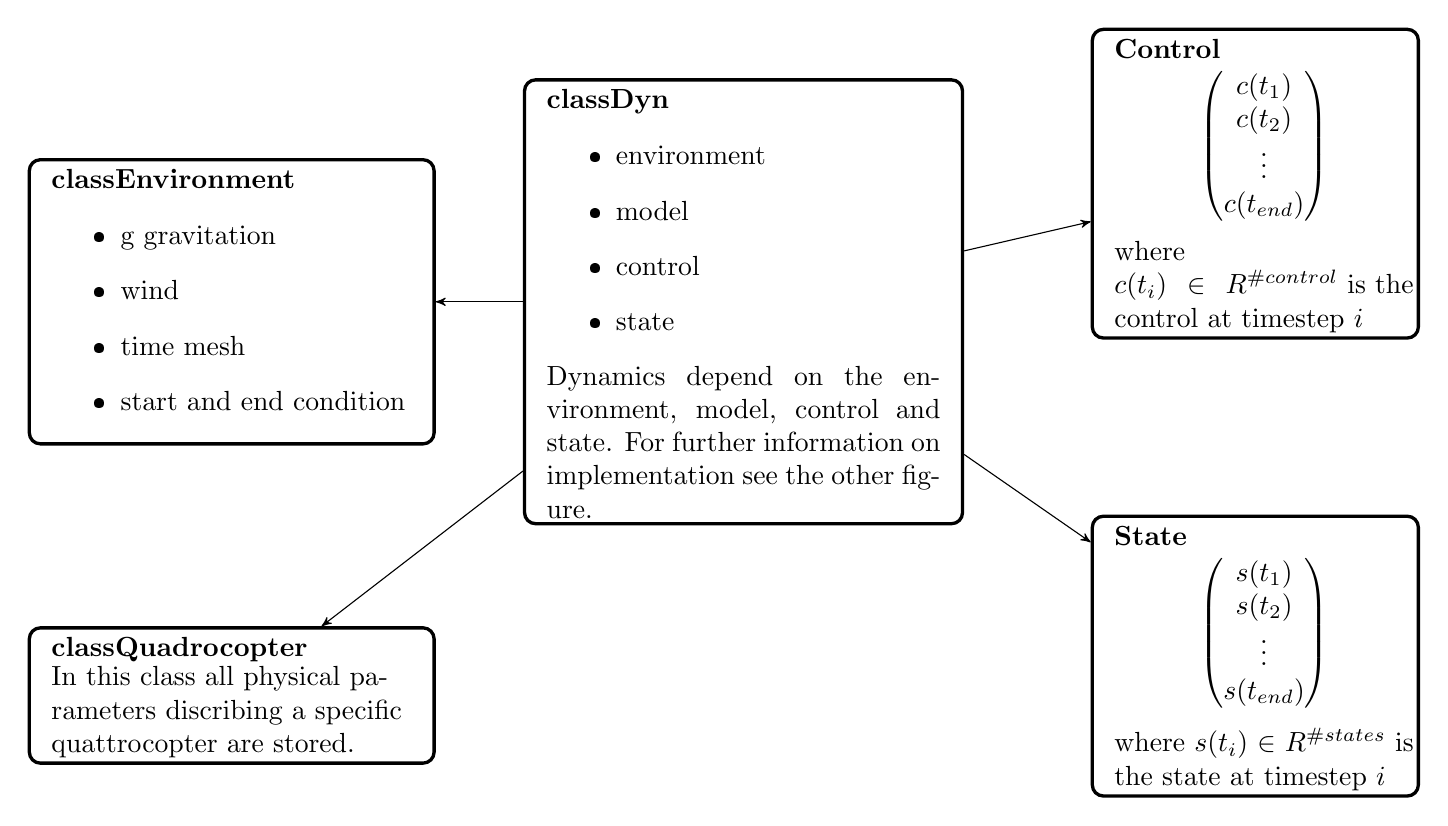
\begin{tikzpicture}[->,>=stealth']

\tikzset{
    state/.style={
           rectangle,
           rounded corners,
           draw=black, very thick,
           minimum height=2em,
           inner sep=2pt,
           text centered,
           },
}
 % Position of classDyn 
 % Use previously defined 'state' as layout (see above)
 % use tabular for content to get columns/rows
 % parbox to limit width of the listing
 \node[state] (classDyn) 
 {\begin{tabular}{l}
  \textbf{classDyn}\\
  \parbox{4cm}{\begin{itemize}
  \item environment
 \item model
\item control 
\item state

  \end{itemize}
  }
\\[4em]
 
  \parbox{5cm}{
Dynamics depend on the environment, model, control and state. For further information on implementation see the other figure.
  }
 \end{tabular}};
  
 \node[state,    	% layout (defined above)
  text width=5cm, 	% max text width
  yshift=0cm, 		% move 2cm in y
  left of=classDyn, 	% Position is to the right of classDyn
  node distance=6.5cm, 	% distance to classDyn
  anchor=center] (classEnv) 	% posistion relative to the center of the 'box'
 {%
 \begin{tabular}{l} 	% content
  \textbf{classEnvironment}\\
  \parbox{4.8cm}{
\begin{itemize}
\item g gravitation
\item wind
\item time mesh
\item start and end condition
\end{itemize}
}
 \end{tabular}
 };
 
 % STATE classCopter
 \node[state,
  below of=classEnv,
  yshift=-4cm,
  anchor=center,
  text width=5cm] (classCopter) 
 {%
 \begin{tabular}{l}
  \textbf{classQuadrocopter}\\
  \parbox{4.8cm}{In this class all physical parameters discribing a specific quattrocopter are stored.}
 \end{tabular}
 };

 \node[state,    	% layout (defined above)
  text width=4cm, 	% max text width
  yshift=1.5cm, 		% move 2cm in y
  right of=classDyn, 	% Position is to the right of classDyn
  node distance=6.5cm, 	% distance to classDyn
  anchor=center] (control) 	% posistion relative to the center of the 'box'
 {%
 \begin{tabular}{l} 	% content
  \textbf{Control}\\
\parbox{3.8cm}{
$$ \begin{pmatrix}
  c(t_1) \\
  c(t_2) \\
  \vdots \\
  c(t_{end})
\end{pmatrix} $$ 
 where \\ $c(t_i) \in \mathds{R}^{\# control}$ is the control at timestep $i$
}
 \end{tabular}
 };


 \node[state,
  below of=control,
  yshift=-5cm,
  anchor=center,
  text width=4cm] (state) 
 {%
 \begin{tabular}{l}
  \textbf{State}\\
  \parbox{3.8cm}{
  $$ \begin{pmatrix}
  s(t_1) \\
  s(t_2) \\
  \vdots \\
  s(t_{end})
\end{pmatrix} $$ 
 where $s(t_i) \in \mathds{R}^{\# states}$ is the state at timestep $i$
}
 \end{tabular}
 };

 
 % draw the paths and and print some Text below/above the graph
 \path 



(classDyn)     	edge[] node[]{}(classCopter)
(classDyn)		 	edge[] node[]{}(classEnv)
(classDyn)			edge[] node[]{}(state)
(classDyn)			edge[] node[]{}(control)
;

\end{tikzpicture}

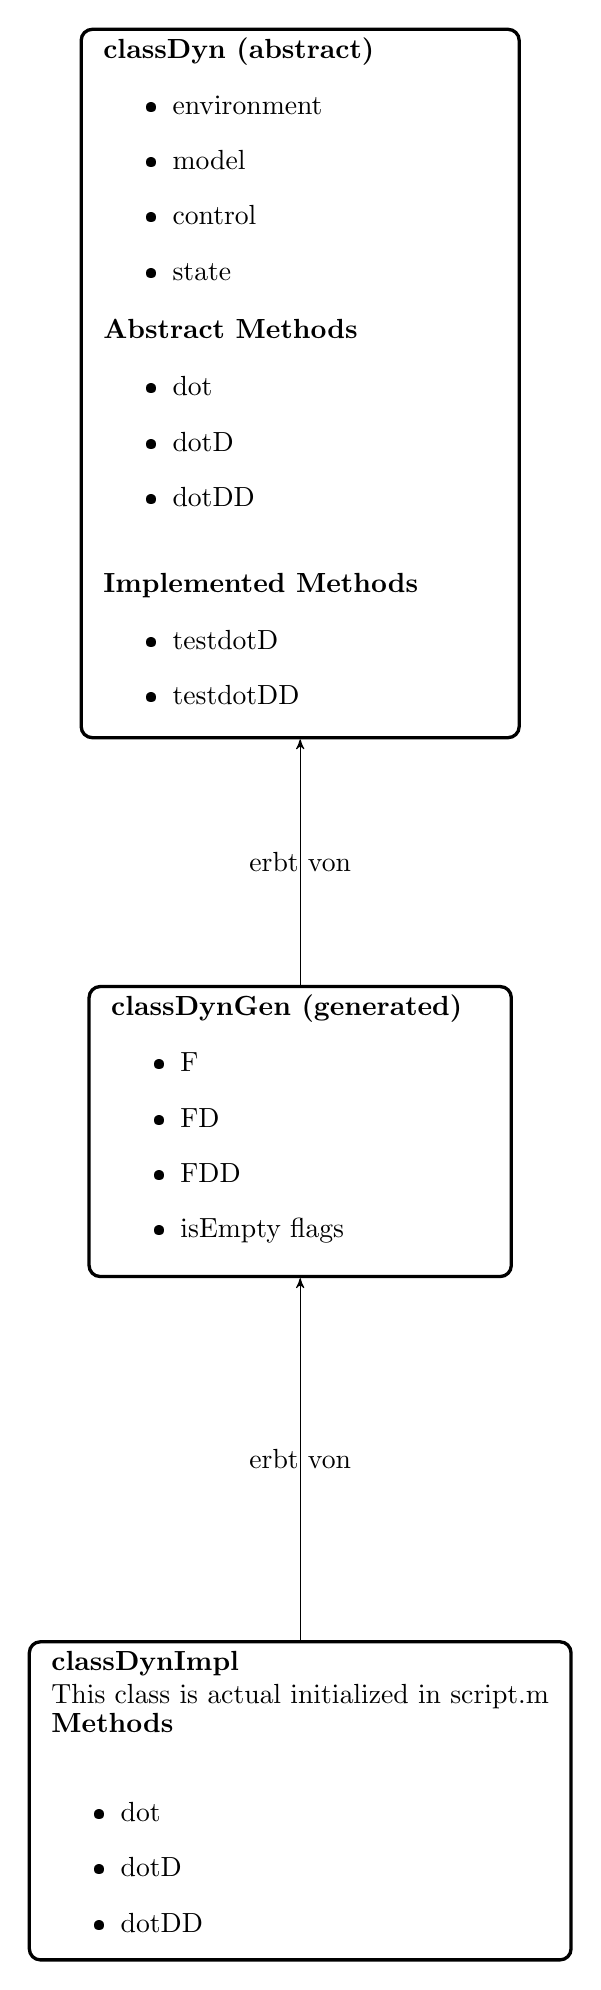
\begin{tikzpicture}[->,>=stealth']

\tikzset{
    state/.style={
           rectangle,
           rounded corners,
           draw=black, very thick,
           minimum height=2em,
           inner sep=2pt,
           text centered,
           },
}
 % Position of classDyn 
 % Use previously defined 'state' as layout (see above)
 % use tabular for content to get columns/rows
 % parbox to limit width of the listing
 \node[state] (classDyn) 
 {\begin{tabular}{l}
  \textbf{classDyn (abstract)}\\
  \parbox{4cm}{\begin{itemize}
  \item environment
 \item model
\item control 
\item state

  \end{itemize}
  }
\\[4em]
\textbf{Abstract Methods} \\
  \parbox{5cm}{
\begin{itemize}
\item dot 
\item dotD
\item dotDD
\end{itemize} 
  }
\\[4em]
\textbf{Implemented Methods} \\
  \parbox{5cm}{
\begin{itemize}
\item testdotD
\item testdotDD
\end{itemize}
}
 \end{tabular}};
  
\node[state,    	% layout (defined above)
  yshift=-3cm, 		% move 2cm in y
  below of=classDyn, 	% Position is to the right of classDyn
  node distance=6.5cm, 	% distance to classDyn
  anchor=center] (classDynGen) 	% posistion relative to the center of the 'box'
 {%
 \begin{tabular}{l} 	% cntent
  \textbf{classDynGen (generated) }\\
  \parbox{4.8cm}{
\begin{itemize}
\item F
\item FD
\item FDD
\item isEmpty flags
\end{itemize}
}
 \end{tabular}
 };

\node[state,    	% layout (defined above)
  yshift=-2cm, 		% move 2cm in y
  below of=classDynGen, 	% Position is to the right of classDyn
  node distance=6.5cm, 	% distance to classDyn
  anchor=center] (classDynImpl) 	% posistion relative to the center of the 'box'
 {%
 \begin{tabular}{l} 	% cntent
  \textbf{classDynImpl  }\\
This class is actual initialized in script.m \\
  \parbox{4.8cm}{
\textbf{Methods}\\
\begin{itemize}
\item dot
\item dotD
\item dotDD
\end{itemize}
}
 \end{tabular}
 };

 
 % draw the paths and and print some Text below/above the graph
 \path 



(classDynGen)     	edge[] node[]{erbt von}(classDyn)
(classDynImpl)		 	edge[] node[]{erbt von}(classDynGen)

;

\end{tikzpicture}


\end{document}